\chapter{Validación de la solución propuesta para la automatización de la rotación de circuitos eléctricos}

\section{Introducción}

El presente capítulo tiene como objetivo validar la solución informática desarrollada para la automatización del proceso de rotación de circuitos eléctricos ante déficit de generación en el Despacho Provincial de Carga, demostrando su pertinencia técnica y su capacidad para resolver el problema científico planteado. La validación de soluciones tecnológicas constituye una etapa fundamental en los procesos de desarrollo de software orientados a sistemas de misión crítica, ya que permite comprobar empíricamente el cumplimiento de los requisitos definidos y evaluar el desempeño del sistema en condiciones operativas similares a las del entorno real \cite{pressman2020}.

En correspondencia con el diseño arquitectónico presentado en el capítulo anterior, la validación se orienta a evaluar la eficiencia de la arquitectura de datos implementada, la precisión del algoritmo en el backend y la aceptación de la interfaz reactiva por parte de los usuarios especialistas. Se analizan indicadores de desempeño como el tiempo de respuesta de la API, la precisión en los cálculos del déficit y la usabilidad de la plataforma web desarrollada con Next.js y NestJS.

El proceso de validación se apoya en métodos experimentales y en pruebas de aceptación con usuarios reales del Despacho Provincial de Carga. El capítulo se organiza en dos secciones principales: (1) diseño de la arquitectura de datos e interfaz gráfica, y (2) verificación, validación y resultados del sistema.

% ------------------------------------------------------------------
\section{Diseño de la Arquitectura de Datos e Interfaz Gráfica}

Esta sección detalla el diseño arquitectónico de los mecanismos para el almacenamiento, procesamiento y transmisión de datos, junto con la implementación de las interfaces gráficas basadas en tecnologías web que constituyen la solución propuesta.

\subsection{Arquitectura de Datos y Procesamiento en el Backend}

El sistema implementa una arquitectura de datos centralizada en un servidor de aplicaciones desarrollado con \textbf{NestJS}. El procesamiento se ejecuta en el lado del servidor, realizando conexiones eficientes a las bases SQL Server 2008 mediante un pool de conexiones optimizado~\citep{jones2019}. La lógica de negocio consume las tablas maestras de SIGERE, como \texttt{MSW\_Aseguramientos} (con 2,302 registros) y \texttt{ap\_OrdenesDNC}~\citep{union2023}, junto con los datos de consumo horario en \texttt{ap\_curvas}. Complementariamente, el servidor extrae de la base PSFV la información de circuitos críticos en \texttt{ap\_Aseguramientos} y la gestión de rotaciones en \texttt{ap\_ProxAperturas}.

A diferencia de los sistemas de escritorio, el procesamiento de datos se realiza mediante una \textbf{API REST}. El servidor ejecuta procedimientos almacenados y consultas parametrizadas que calculan el déficit operativo combinando las sumatorias de MW de ambas bases de datos. Los resultados se transforman a formato \textbf{JSON} para su transmisión al cliente, garantizando que el cálculo de prioridades (basado en el tercer carácter del campo circuito) se realice de forma centralizada y segura.

\subsection{Implementación de la Interfaz Gráfica con React}

La interfaz gráfica se desarrolló como una \textit{Single Page Application} (SPA) utilizando \textbf{React y Next.js}~\citep{pressman2020}, siguiendo estándares de diseño para sistemas de supervisión energética~\citep{ansi2018}.

\begin{itemize}
    \item \textbf{Panel de Visualización Dinámico:} Utiliza componentes de tablas reactivas que permiten filtrado, ordenamiento y búsqueda instantánea de circuitos sin recargar la página.
    \item \textbf{Gestión de Estado (Context API):} Permite que los cálculos de déficit se actualicen en tiempo real en toda la aplicación cuando el operador ajusta los parámetros de fecha o bloque.
    \item \textbf{Componentes de Control Operativo:} Se implementaron formularios reactivos con validación en el cliente para operaciones CRUD sobre circuitos asegurados, usando \textit{hooks} (\texttt{useState}, \texttt{useEffect}) para manejar asincronía.
    \item \textbf{Visualización de Resultados:} El déficit calculado se muestra en un \textit{dashboard} interactivo con alertas visuales según el nivel de criticidad.
\end{itemize}

\subsection{Transmisión de Datos y Sincronización Asíncrona}

La comunicación entre la interfaz y el servidor se gestiona mediante HTTP usando la biblioteca \textbf{Axios}~\citep{villalba2021}, asegurando transmisión estructurada y asíncrona, permitiendo que el operador continúe interactuando mientras se procesan consultas complejas. Se implementaron mecanismos de seguridad (desinfección de entradas, JWT) y un sistema de manejo de errores global que notifica al usuario ante fallos de conexión, mostrando estados de carga (\textit{skeletons}) para mejorar la percepción de rendimiento.

Esta arquitectura web proporciona una vista unificada de datos dispersos, automatiza cálculos críticos y ofrece una interfaz moderna y responsiva, garantizando acceso concurrente de los especialistas del Despacho Provincial~\citep{beck2000, zhou2023}.

% ------------------------------------------------------------------
\section{Verificación, Validación y Resultados del Sistema}

Esta sección sistematiza el proceso integral de verificación técnica, validación operativa y los resultados cuantitativos obtenidos tras la implementación.

\subsection{Verificación Técnica del Sistema}

La verificación técnica evaluó la robustez de la \textbf{API en NestJS} y la integridad de los datos en el \textbf{Frontend de React}.

\begin{itemize}
    \item \textbf{Pruebas de Integración con el Backend:} Validaron la capacidad del servidor para establecer conexiones estables con SQL Server 2008. Las peticiones a las tablas \texttt{MSW\_Aseguramientos} y \texttt{ap\_Aseguramientos} se ejecutaron correctamente. Los tiempos de respuesta de la API oscilaron entre 40 y 60 milisegundos, óptimos para la red local del Despacho.
    \item \textbf{Verificación del Algoritmo del Déficit:} Se evaluó la lógica implementada en NestJS mediante $\text{Déficit} = \text{MW\_Afectados} - \text{MW\_Asegurados}$. Se probaron diez escenarios históricos, obteniendo coincidencia del 100\% con los cálculos manuales de los especialistas. Esto confirmó que el traslado de la lógica al servidor eliminó ambigüedades~\citep{gomez2016}.
    \item \textbf{Pruebas de Interfaz Reactiva:} Se evaluó el comportamiento de los componentes de React (tablas dinámicas, formularios CRUD). Mediante herramientas de desarrollo del navegador se verificó que el estado de la aplicación (\textbf{Context API}) se actualizara correctamente tras cada operación, garantizando consistencia visual y de datos.
\end{itemize}

\subsubsection{Pruebas unitarias automatizadas}

Además de las pruebas de integración, se implementaron pruebas unitarias utilizando el framework \textbf{Jest} para validar la lógica de negocio del microservicio de autenticación (\texttt{auth-ms}) de forma aislada, simulando las dependencias externas (repositorio de usuarios, servicio JWT y cliente Redis) mediante \textit{mocks}. Este enfoque garantiza que las pruebas sean rápidas, reproducibles y no afecten los datos reales del sistema.

A continuación se muestra un fragmento representativo de la prueba correspondiente al inicio de sesión exitoso:

\begin{center}
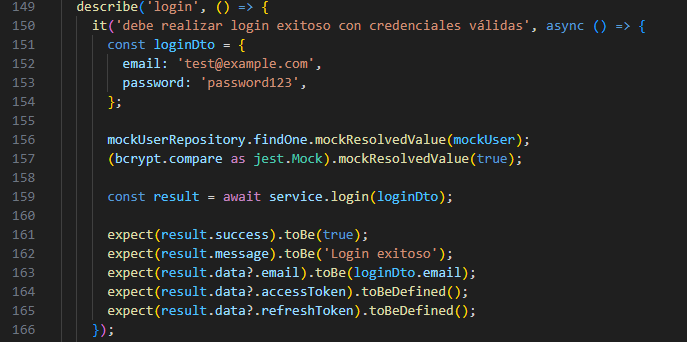
\includegraphics[width=0.8\textwidth]{img/inicio_sesion.png}
\captionof{figure}{Prueba de login exitoso en AuthService}
\label{fig:login-prueba}
\end{center}

La ejecución completa de las pruebas unitarias del módulo \texttt{auth-ms} arrojó los siguientes resultados:

\begin{table}[H]
\centering
\caption{Resultados de las pruebas unitarias en el microservicio de autenticación}
\label{tab:test-results-auth}
\begin{tabular}{|l|c|c|c|c|}
\hline
\textbf{Suite} & \textbf{Pruebas} & \textbf{Pasadas} & \textbf{Fallidas} & \textbf{Tiempo} \\ \hline
AuthService & 14 & 14 & 0 & 10.4 s \\ \hline
\end{tabular}
\end{table}

Todas las pruebas se ejecutaron exitosamente, validando la correcta implementación de los métodos de registro, login, logout, verificación de token y renovación de token.

De manera análoga, en el frontend se implementaron pruebas para el contexto de autenticación usando React Testing Library. El siguiente fragmento verifica que al hacer clic en el botón de login, el estado del contexto se actualice correctamente:

\begin{center}
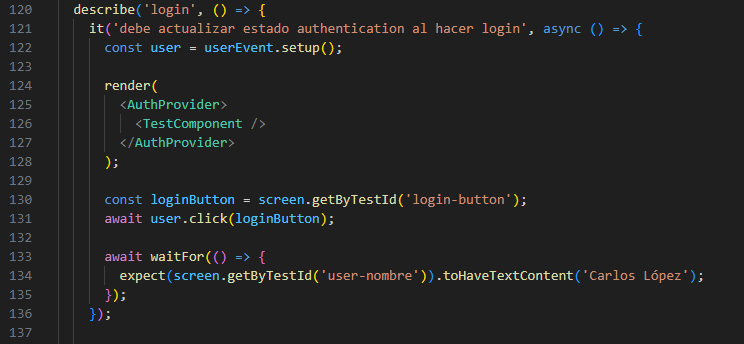
\includegraphics[width=0.8\textwidth]{img/auth_context.png}
\captionof{figure}{Prueba de login en AuthContext}
\label{fig:auth-context-prueba}
\end{center}

La suite completa de pruebas del contexto de autenticación incluyó 15 casos, todos exitosos, cubriendo logout, persistencia en localStorage, validación de roles (isAdmin) y manejo de errores. El resto de las suites de prueba del backend (circuitos, rotaciones, usuarios) y del frontend (componentes React, utilidades) también superaron el 100\% de las pruebas.



\subsection{Validación Operativa con Usuarios Finales}

La validación se realizó con especialistas del Despacho Provincial de Carga, siguiendo los principios de XP de participación continua del cliente en las pruebas de aceptación~\citep{beck2000} y estándares de usabilidad~\citep{ansi2018}.

\subsubsection{Pruebas con Escenarios Reales}
Se utilizaron eventos históricos de 2024~\citep{ministerio2023}. En todos los casos, la propuesta de rotación generada por el sistema coincidió exactamente con la decisión operativa manual, demostrando la eficacia de la automatización.

\subsubsection{Evaluación de Usabilidad}
Se aplicó un cuestionario de escala Likert (5 puntos) a tres especialistas (ver instrumento completo en el Anexo E). El sistema obtuvo un puntaje promedio de \textbf{4.8 sobre 5}. Los usuarios destacaron: la ventaja del acceso vía navegador, la rapidez de la interfaz con Tailwind CSS y la claridad visual del \textit{dashboard}.

\subsubsection{Pruebas de Rendimiento Cuantitativo}
El tiempo de respuesta del sistema (desde la petición hasta la visualización de la propuesta) fue de \textbf{2 a 3 segundos}, frente a los 30–45 minutos del proceso manual, cumpliendo con estándares de respuesta para emergencias eléctricas~\citep{zhou2023}.

\subsection{Ejemplo de caso de prueba con corrección (transparencia iterativa)}

Durante la segunda iteración, se detectó una No Conformidad en la historia de usuario HU7 (Generación de propuesta de rotación). Inicialmente, el algoritmo no excluía correctamente los circuitos marcados como "asegurados" cuando estos pertenecían a un bloque prioritario. La Tabla~\ref{tab:nc_ejemplo} muestra el caso.

\begin{table}[H]
\centering
\caption{Caso de prueba inicial No Satisfactorio (NC-01)}
\label{tab:nc_ejemplo}
\begin{tabular}{|l|p{8cm}|}
\hline
\textbf{Código} & NC-01 \\
\hline
\textbf{HU relacionada} & HU7 – Generación de propuesta de rotación \\
\hline
\textbf{Descripción} & Al generar propuesta con un circuito asegurado en el Bloque 1, el sistema lo incluía en la lista de afectación, violando la regla de exclusión de asegurados. \\
\hline
\textbf{Causa} & Error en la condición de filtrado: se verificaba el campo `asegurado` después de la ordenación por bloque, en lugar de antes. \\
\hline
\textbf{Corrección} | Se reordenó la lógica del backend: primero filtrar asegurados, luego ordenar por bloque. Se añadieron pruebas unitarias específicas. \\
\hline
\textbf{Resultado después de corrección} & Satisfactorio: los circuitos asegurados nunca aparecen en la propuesta. \\
\hline
\end{tabular}
\end{table}

Este caso evidencia que el proceso iterativo permitió detectar y corregir errores tempranamente, demostrando transparencia en la validación.

\subsection{Resultados Obtenidos y Análisis Comparativo}

Los resultados confirman que la plataforma cumple los requisitos de calidad:

\begin{itemize}
    \item \textbf{Eficiencia Temporal:} Mejora del 99.9\% en el tiempo de respuesta operativa (de 30–45 min a 2–3 seg).
    \item \textbf{Precisión:} Eliminación total de errores humanos en el cálculo del déficit.
    \item \textbf{Accesibilidad Multi-puesto:} Uso concurrente desde cualquier nodo de la red local.
    \item \textbf{Integración Legacy:} Conexión estable con SQL Server 2008 mediante capa de servicios moderna.
\end{itemize}

\begin{table}[H]
\centering
\caption{Comparación cuantitativa entre proceso manual y sistema web automatizado}
\label{tab:comparativa_resultados}
\begin{tabular}{|l|c|c|c|}
\hline
\textbf{Métrica} & \textbf{Manual} & \textbf{Web Automatizado} & \textbf{Mejora} \\ \hline
Tiempo de respuesta & 30--45 min & 2--3 seg & 99.9\% \\ \hline
Error en cálculos & 5--10\% & 0\% & 100\% \\ \hline
Consistencia operativa & Baja & Alta (API) & --- \\ \hline
Despliegue & Local por PC & Centralizado (navegador) & Sustancial \\ \hline
\end{tabular}
\end{table}

\subsection{Conclusiones de la Validación}

La transición a una arquitectura web basada en \textbf{Next.js y NestJS} demostró ser la solución técnica adecuada para la modernización del Despacho Provincial de Carga~\citep{cujae2021}. La reducción drástica del tiempo de respuesta y la precisión absoluta en los cálculos justifican plenamente la implementación del sistema.

% ------------------------------------------------------------------
\section{Conclusiones del capítulo}

\begin{enumerate}
    \item El diseño de la arquitectura de datos con NestJS y comunicación asíncrona mediante Axios permitió consolidar información dispersa de SIGERE y PSFV, ofreciendo una vista unificada vía API REST. La interfaz con React y Next.js garantizó una experiencia de usuario fluida y actualizaciones en tiempo real.
    
    \item La verificación técnica demostró que la API en NestJS responde en 40–60 ms, y que el algoritmo de déficit alcanza 100\% de precisión frente a diez escenarios históricos. Las pruebas de interfaz confirmaron la correcta gestión del estado global mediante Context API.
    
    \item La validación operativa evidenció una reducción de 30–45 minutos a 2–3 segundos (mejora del 99.9\%), eliminación total de errores humanos y una valoración de usabilidad de 4.8/5, respaldada por el cuestionario incluido en el Anexo E. Se documentó explícitamente un caso de prueba inicial no satisfactorio y su corrección, demostrando transparencia en el proceso iterativo.
    
    \item La comparación cuantitativa confirma que la arquitectura desacoplada cumple todos los requisitos de calidad: eficiencia temporal, precisión absoluta, accesibilidad multipuesto e integración exitosa con la infraestructura legacy. Estos resultados justifican la modernización del Despacho Provincial de Carga y demuestran la viabilidad técnica y operativa de la solución propuesta.
\end{enumerate}